\documentclass[12pt]{beamer}

\usepackage{graphicx}

\title{The Effect of Aesthetic on the Usability of Data Visualization}
\subtitle{Nick Cawthon and Andrew Vande Moere, IEEE 2007}
\author{Brian To}

\begin{document}
  \maketitle

  \begin{frame}{Motivations}
    \begin{itemize}
      \item Aesthetics is an under-represented field in data visualization.
            % Talk about "typical" data visualization topics
      \item Aesthetically-pleasing visualizations improve the \emph{efficiency}
            and \emph{effectiveness} of a task.
            % Say "sounds weird, but there's previous research on it"
            % Give plausible explanation
      \item Hypothesis: Task Abandonment and Erroneous Response Latency are
            related to aesthetics.
            % Say "they are taking an existing conclusion and trying to augment
            % it"
      \item Purpose of this paper is to emphasize the importance of aesthetics
            in data visualization and analysis.
            % Say "think of it as a persuasive essay, but as research"
    \end{itemize}
  \end{frame}

  \begin{frame}{Experimental Design}
    \begin{itemize}
      \item Online Survey
            % b/c * Similar to existing web study
            %     * Easiest way to collet buttloads of datas
      \item Aesthetic Ranking and Task Performance
      \item Group and Individual aesthetic rankings
      \item Tracked demographic information (age, gender, language)
      \item Collected proportion correct, abandoned, and response times for
            incorrect, correct, and abandoned.
            % Also mention randomization
    \end{itemize}
  \end{frame}
      
  \begin{frame}{Experimental Design}
    \begin{itemize}
      \item One data set, 11 possible visualizations
            % Hierarchical data set of folders
            
            % Aesthetic - "on this scale, how does it rank?"
            % Task Perf - questions
      \item Color, Size, Scale, Position, and Typography kept constant
    \end{itemize}
    
    \begin{center}
      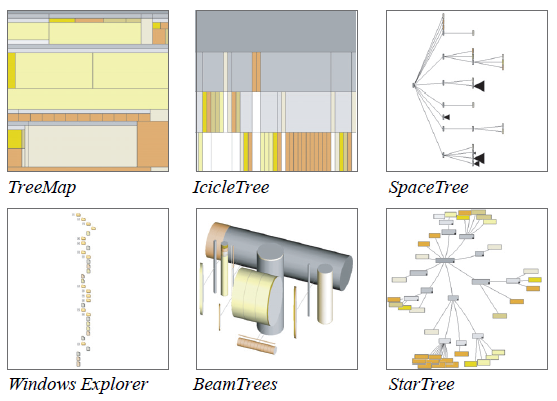
\includegraphics[scale=0.5]{visualizations.png}
    \end{center}
  \end{frame}

  \begin{frame}{Conclusions}
    \begin{itemize}
      \item Beautiful does not imply efficient.
      \item Similar visualizations did not recieve similar scores.
      \item More aesthetic visualizations had longer erroneous response times
            and a lower task abandonment rate.
    \end{itemize}
  \end{frame}
  
  \begin{frame}{Discussion}
    \begin{itemize}
      \item Some visualizations are better suited to different kinds of data.
      \item The earthen-colored pallette is aesthetically pleasing (according
            to Tufte). This may have equalized ranking in attractiveness.
      \item Some visualizations are better with interaction, which may have
            confounded with results.
    \end{itemize}
  \end{frame}
  
  \begin{frame}{Relevance}
    \begin{quote}
      It is only through our emotions do we unravel problems, as the human
      emotional system is intertwined with our cognitive abilities.
      
      -- Donald A. Norman
    \end{quote}
  \end{frame}
\end{document}